The Computing Platform, mounted on the multirotor, is comprised of two distinct processing platforms: the \textit{Platform Management Board} (PMB) and the \textit{Programmable Logic Board} (PLB). The PMB hosts the software and interfaces required to interface with both the PMB (also present on the multirotor) and the base station.

\begin{figure}[H]\label{hlpic}
    \centering
    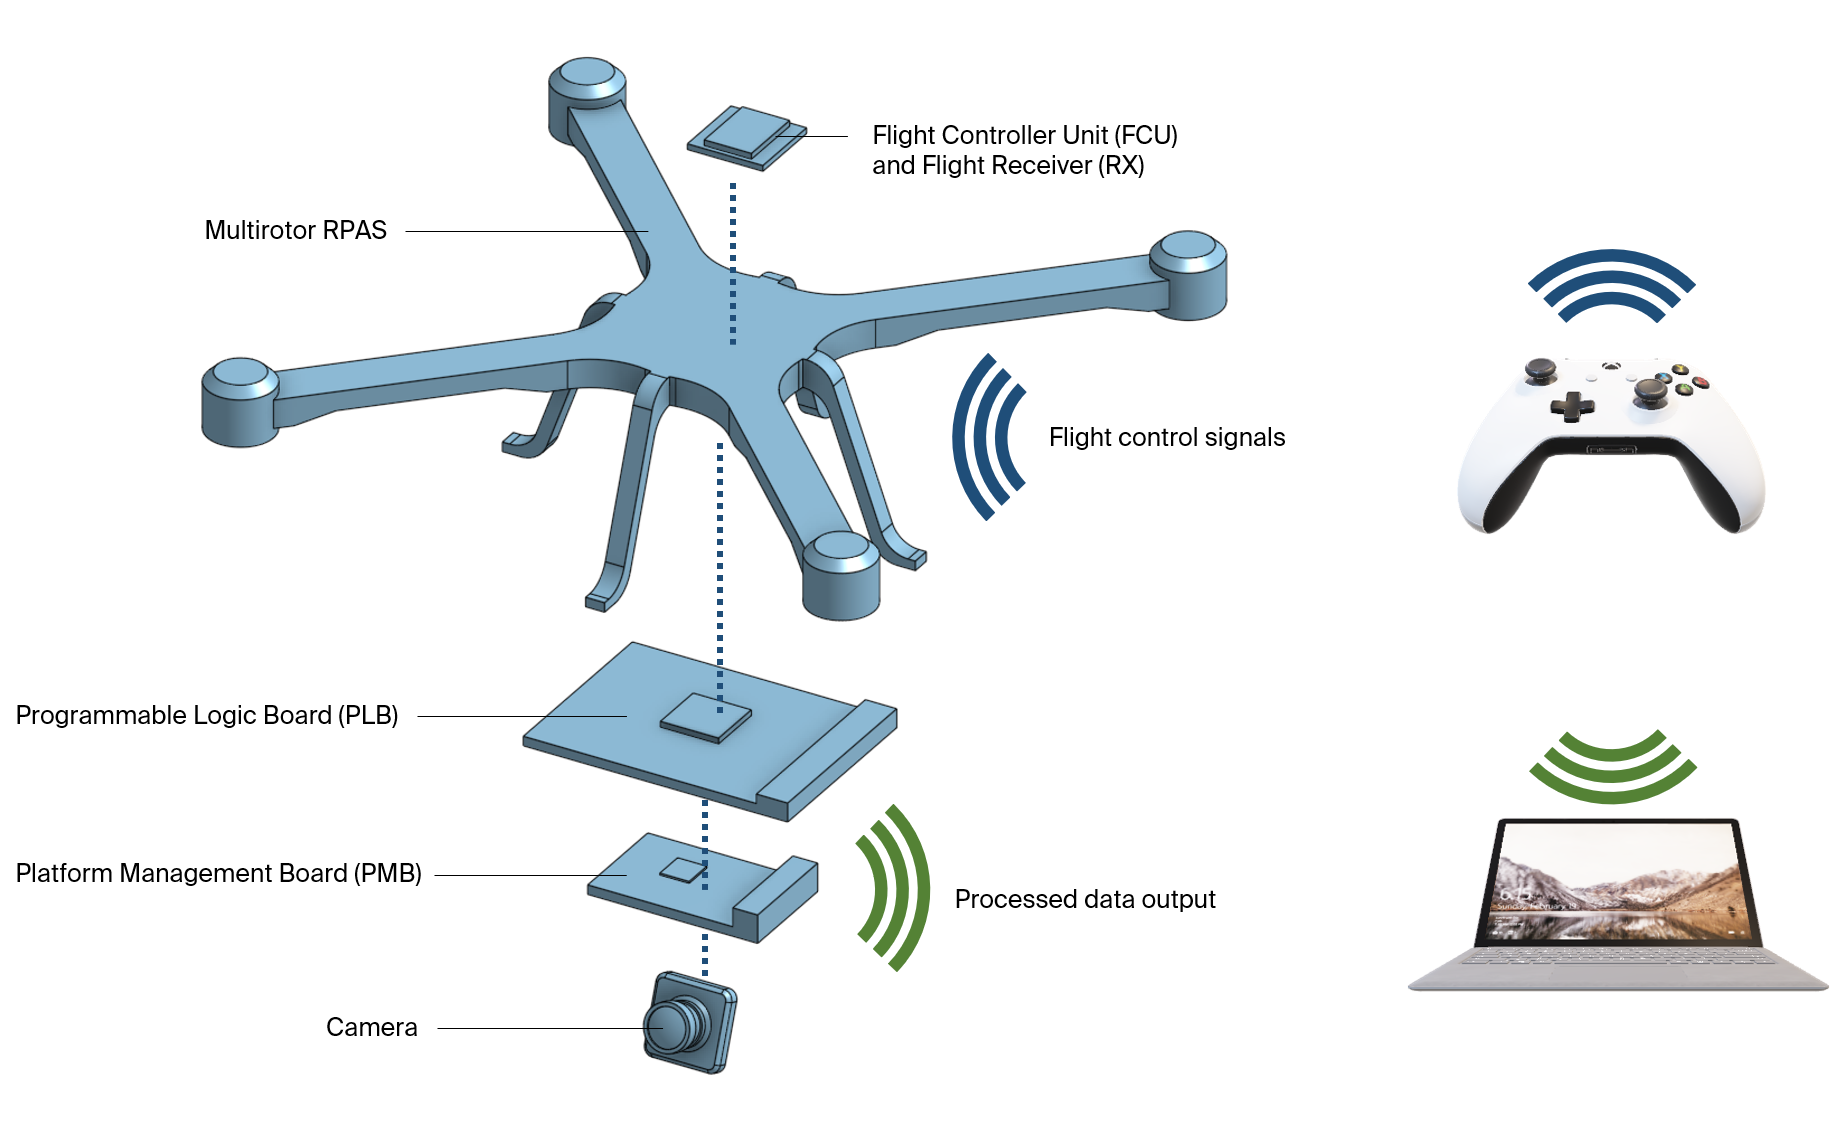
\includegraphics[width=\linewidth]{img/intpic}
\caption{High-Level System Integration with RPAS}
\end{figure}

\begin{figure}[H]\label{hldiag}
\centering
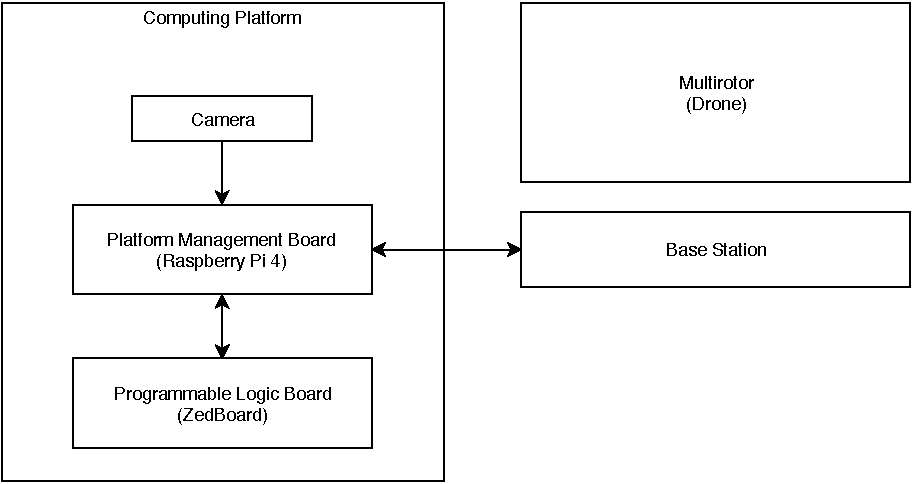
\includegraphics[width=15cm]{img/highlevel.pdf}
\caption{High-Level System Architecture}
\end{figure}

